\documentclass[12pt,a4paper]{article}
\usepackage[utf8]{inputenc}
\usepackage{amsmath}
\usepackage[brazilian]{babel}
\usepackage{breqn}
\usepackage{amsfonts}
\usepackage{amssymb}
\usepackage{graphicx}
\usepackage[margin=0.8in]{geometry}


\begin{document}
\title{\vspace{70mm}\Huge Experimento 03 - Ondas Estacionárias}
\author{ Giovani Garuffi\qquad\hfill
		\textit {RA: 155559}\protect\\
		João Baraldi\hfill
		\textit{RA: 158044}\protect\\
		Lauro Cruz\hfill
		\textit{RA: 156175}\protect\\
		Lucas Schanner\hfill
		\textit{RA: 156412}\protect\\
		Pedro Stringhini\hfill
		\textit {RA: 156983}								
		}
\maketitle
\newpage
\section{Resumo}

\section{Objetivos}


\section{Procedimento Experimental e Coleta de Dados}

\subsection{Materiais utilizados}


\subsection{Procedimento}




\subsection{Dados Obtidos}







\section{Análise dos Resultados e Discussões}
\subsection{Linearização}
A equação
$$ L = \dfrac{1}{2f} \sqrt{\dfrac{mg}{\mu}} n $$
Pode ser reescrita como
$$ L = (\dfrac{1}{2f} \sqrt{\dfrac{g}{\mu}}) \cdot n\sqrt{m} $$
Vemos então que deve existir uma uma relação linear entre $L$ e $n\sqrt{m}$ em que o coeficiente angular é $a = \dfrac{1}{2f} \sqrt{\dfrac{g}{\mu}}$ e o coeficiente linear é $b = 0$, que pode ser verificada utilizando-se a tabela abaixo:

\begin{table}[!htbp]
\centering
\def\arraystretch{1.3}
\caption{Valores de $m$, $\sqrt{m}$ e $n\sqrt{m}$ relacionados aos comprimentos do fio $L$}
\label{Resultados}
\begin{tabular}{|l|c|c|c|c|}
\hline
$L$ $(m)$ & $n$ & $m$ $(Kg)$ & $\sqrt{m}$ $(\sqrt{Kg})$ & $n\sqrt{m}$ $(\sqrt{Kg})$ \\
\hline
$0.875\pm0.001$ & $2$ & $0.2586\pm0.0001$ & $0.5085\pm0.0001$ & $1.0171\pm0.0002$ \\
\hline
$0.905\pm0.001$ & $4$ & $0.0718\pm0.0001$ & $0.2680\pm0.0002$ & $1.0718\pm0.0007$ \\
\hline
$0.973\pm0.001$ & $5$ & $0.0498\pm0.0001$ & $0.2232\pm0.0002$ & $1.116\pm0.001$ \\
\hline
$0.985\pm0.001$ & $3$ & $0.1975\pm0.0001$ & $0.4444\pm0.0001$ & $1.3332\pm0.0003$ \\
\hline
$1.065\pm0.001$ & $4$ & $0.1042\pm0.0001$ & $0.3228\pm0.0002$ & $1.2912\pm0.0006$ \\
\hline
$1.155\pm0.001$ & $5$ & $0.0718\pm0.0001$ & $0.2680\pm0.0002$ & $1.3400\pm0.0009$ \\
\hline
$1.168\pm0.001$ & $6$ & $0.0498\pm0.0001$ & $0.2232\pm0.0002$ & $1.340\pm0.001$ \\
\hline
$1.193\pm0.001$ & $3$ & $0.2322\pm0.0001$ & $0.4819\pm0.0001$ & $1.4456\pm0.0003$ \\
\hline
$1.255\pm0.001$ & $3$ & $0.2586\pm0.0001$ & $0.5085\pm0.0001$ & $1.5256\pm0.0003$ \\
\hline
$1.300\pm0.001$ & $7$ & $0.0498\pm0.0001$ & $0.2232\pm0.0002$ & $1.562\pm0.002$ \\
\hline
$1.310\pm0.001$ & $4$ & $0.1975\pm0.0001$ & $0.4444\pm0.0001$ & $1.7776\pm0.0004$ \\
\hline
$1.340\pm0.001$ & $5$ & $0.1042\pm0.0001$ & $0.3228\pm0.0002$ & $1.6140\pm0.0008$ \\
\hline
$1.365\pm0.001$ & $6$ & $0.0718\pm0.0001$ & $0.2680\pm0.0002$ & $1.608\pm0.001$ \\
\hline

\end{tabular} \\

\end{table}

\subsection{Regressão linear}
Fazendo-se a regressão linear $n\sqrt{m}$ por $L$ obtem-se os coeficientes:
$$a = 1.3985 \pm 0.0007 \dfrac{m}{\sqrt{Kg}}$$
$$b = -0.196 \pm 0.001 m$$
Sendo $a$ o coeficiente angular e $b$ o coeficiente linear.
Nota-se que segundo a linearização da equação original, o coeficiente linear deveria ser nulo, o que não condiz com a regressão linear dos dados experimentais. Isso se deve a erros aleatórios e erros durante as medições.
A sobreposição da reta obtida sobre os pontos da tabela pode ser vista no gráfico abaixo:

\begin{figure} [!htbp]

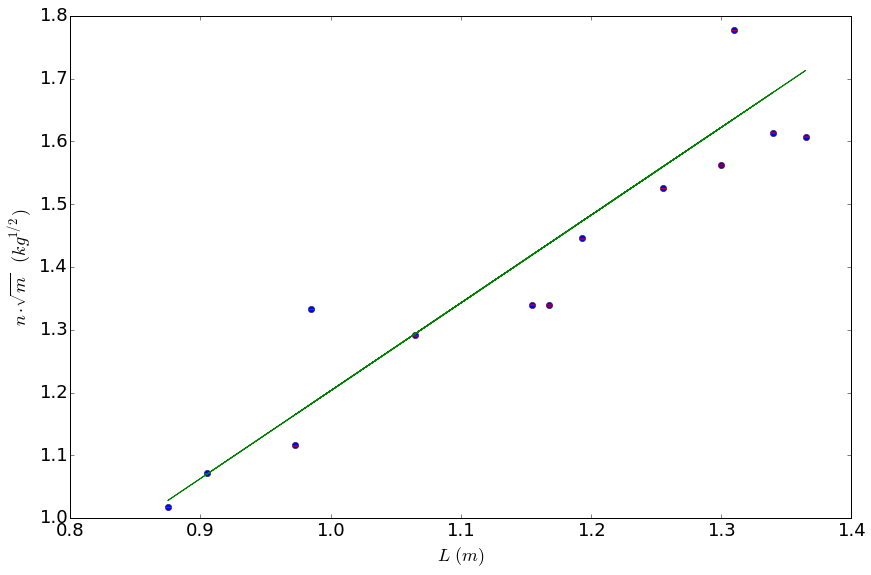
\includegraphics[scale=0.6]{graf1.png}
\caption{Gráfico da regressão linear de $n\sqrt{m}$ por $L$, sobreposta aos pontos obtidos experimentalmente.}

\end{figure}
\subsection{Densidade linear do fio}
A densidade linear do fio é a relação entre o comprimento ($L$) do fio e sua massa ($M_f$), representado por $\mu = \dfrac{M_f}{L}$.\\\\
A representação física do coeficiente linear ($a$) é:
$$a = \dfrac{1}{2f} \sqrt{\dfrac{g}{\mu}}$$
Isolando $\mu$ obtemos:
$$ \mu = \dfrac{g}{4a^2f^2} $$
Fazendo as devidas substituições:
$$ \mu = $$
O erro de $\mu$ é dado por:
$$ \Delta \mu = \dfrac{g}{2f^2a^3} \Delta a $$
Fazendo as devidas substituições:
$$\Delta \mu = $$

\section{Conclusões}


\begin{thebibliography}{9}


\end{thebibliography}

\end{document}

